\documentclass[11pt, a4paper, twoside, openright]{article} 

\usepackage{graphicx,color}
\usepackage{amssymb, amsmath, array, cite, float, url}



\begin{document}

% Example of title page for the projects carried out within DEDIS
% Copied from lasec 

% Simply include it in your mastex tex file: 
%        % Example of title page for the projects carried out within DEDIS
% Copied from lasec 

% Simply include it in your mastex tex file: 
%        % Example of title page for the projects carried out within DEDIS
% Copied from lasec 

% Simply include it in your mastex tex file: 
%        \input{cover}


% Updated October 2016


\newcommand{\logoepfl}[0]{
  \begin{center}
    
\includegraphics[width=4cm]{logo_epfl_coul.eps}
  \end{center}
  \vspace{0.3cm}
  \hrule
}
\newcommand{\project}[1]{
  \begin{center}
    \large{#1}
  \end{center}
  \vspace{1cm}
}
\newcommand{\department}[1]{
  \begin{center}
    \large{#1}
  \end{center}
}
\newcommand{\lab}[1]{
  \begin{center}
    \large{#1}
  \end{center}
}
\newcommand{\supervisor}[3]{
  \begin{center}
    \begin{normalsize}{
        \bf #1}\\#2\\#3
    \end{normalsize}
  \end{center}
}
\renewcommand{\author}[1]{
  \begin{center}
    \Large{#1}
  \end{center}
  \vspace{0.5cm}
}
\renewcommand{\title}[1]{
  \vspace{3cm}
  \begin{center}
    \huge{#1}
  \end{center}
  \vspace{1.7cm}
}
\renewcommand{\date}[2]{
  \begin{center}
    \normalsize{#1 #2}
  \end{center}
  \vspace{0.5cm}
}


\thispagestyle{empty}


% begin title page
  \logoepfl
  
  \title{Locality-Preserving Blockchain Implementation}
  
  \author{Maxime Sierro}
  \department{School of Computer and Communication Sciences}
  \lab{Decentralized and Distributed Systems lab}
  \project{Bachelor Semester Project}
  
  \date{June}{2019}

  \begin{center}
    \begin{tabular}{cc}
      \begin{tabular}{p{4.0cm}}
        \supervisor{Responsible}{Prof. Bryan Ford}{EPFL / DEDIS}
      \end{tabular}&
      \begin{tabular}{p{4.0cm}}
        \supervisor{Supervisors}{Cristina Basescu, Kelong Cong}{EPFL / DEDIS}
      \end{tabular}
    \end{tabular}
  \end{center}

% end title page




% Updated October 2016


\newcommand{\logoepfl}[0]{
  \begin{center}
    
\includegraphics[width=4cm]{logo_epfl_coul.eps}
  \end{center}
  \vspace{0.3cm}
  \hrule
}
\newcommand{\project}[1]{
  \begin{center}
    \large{#1}
  \end{center}
  \vspace{1cm}
}
\newcommand{\department}[1]{
  \begin{center}
    \large{#1}
  \end{center}
}
\newcommand{\lab}[1]{
  \begin{center}
    \large{#1}
  \end{center}
}
\newcommand{\supervisor}[3]{
  \begin{center}
    \begin{normalsize}{
        \bf #1}\\#2\\#3
    \end{normalsize}
  \end{center}
}
\renewcommand{\author}[1]{
  \begin{center}
    \Large{#1}
  \end{center}
  \vspace{0.5cm}
}
\renewcommand{\title}[1]{
  \vspace{3cm}
  \begin{center}
    \huge{#1}
  \end{center}
  \vspace{1.7cm}
}
\renewcommand{\date}[2]{
  \begin{center}
    \normalsize{#1 #2}
  \end{center}
  \vspace{0.5cm}
}


\thispagestyle{empty}


% begin title page
  \logoepfl
  
  \title{Locality-Preserving Blockchain Implementation}
  
  \author{Maxime Sierro}
  \department{School of Computer and Communication Sciences}
  \lab{Decentralized and Distributed Systems lab}
  \project{Bachelor Semester Project}
  
  \date{June}{2019}

  \begin{center}
    \begin{tabular}{cc}
      \begin{tabular}{p{4.0cm}}
        \supervisor{Responsible}{Prof. Bryan Ford}{EPFL / DEDIS}
      \end{tabular}&
      \begin{tabular}{p{4.0cm}}
        \supervisor{Supervisors}{Cristina Basescu, Kelong Cong}{EPFL / DEDIS}
      \end{tabular}
    \end{tabular}
  \end{center}

% end title page




% Updated October 2016


\newcommand{\logoepfl}[0]{
  \begin{center}
    
\includegraphics[width=4cm]{logo_epfl_coul.eps}
  \end{center}
  \vspace{0.3cm}
  \hrule
}
\newcommand{\project}[1]{
  \begin{center}
    \large{#1}
  \end{center}
  \vspace{1cm}
}
\newcommand{\department}[1]{
  \begin{center}
    \large{#1}
  \end{center}
}
\newcommand{\lab}[1]{
  \begin{center}
    \large{#1}
  \end{center}
}
\newcommand{\supervisor}[3]{
  \begin{center}
    \begin{normalsize}{
        \bf #1}\\#2\\#3
    \end{normalsize}
  \end{center}
}
\renewcommand{\author}[1]{
  \begin{center}
    \Large{#1}
  \end{center}
  \vspace{0.5cm}
}
\renewcommand{\title}[1]{
  \vspace{3cm}
  \begin{center}
    \huge{#1}
  \end{center}
  \vspace{1.7cm}
}
\renewcommand{\date}[2]{
  \begin{center}
    \normalsize{#1 #2}
  \end{center}
  \vspace{0.5cm}
}


\thispagestyle{empty}


% begin title page
  \logoepfl
  
  \title{Locality-Preserving Blockchain Implementation}
  
  \author{Maxime Sierro}
  \department{School of Computer and Communication Sciences}
  \lab{Decentralized and Distributed Systems lab}
  \project{Bachelor Semester Project}
  
  \date{June}{2019}

  \begin{center}
    \begin{tabular}{cc}
      \begin{tabular}{p{4.0cm}}
        \supervisor{Responsible}{Prof. Bryan Ford}{EPFL / DEDIS}
      \end{tabular}&
      \begin{tabular}{p{4.0cm}}
        \supervisor{Supervisors}{Cristina Basescu, Kelong Cong}{EPFL / DEDIS}
      \end{tabular}
    \end{tabular}
  \end{center}

% end title page



\newpage
\setcounter{page}{1}
\tableofcontents
\newpage
        

\section{Introduction}
The goal of this project is to create a blockchain implementation in the context of the locality-focused Nyle system, which is treated in more detail in section \ref{Nyle}.

The implementation is done with DEDIS Lab's Cothority platform, written in Go. The consensus layer is based on ByzCoinX \cite{byzcoinx} which uses a practical Byzantine fault tolerance algorithm \cite{castro1999practical} and is already implemented. For this reason, the project is more focused on the higher layers, such as the sending and storing of transactions and signatures. Those functionalities, however, are implemented from scratch. 

\subsection{Nyle}
\label{Nyle}

\begin{figure}[htbp]
 \centering
  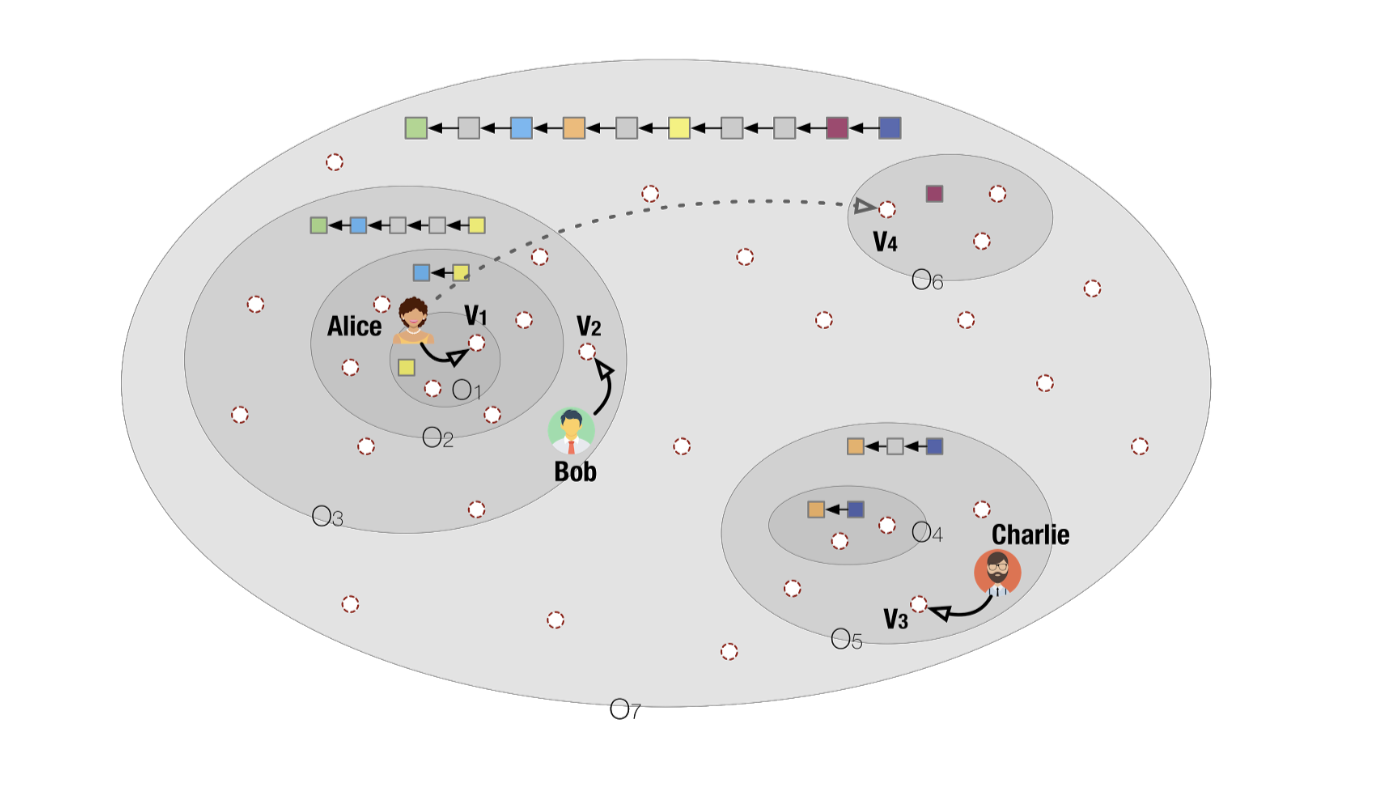
\includegraphics[width=12cm]{nyle.png}
  \caption{Schematic of a Nyle network}
\end{figure}

Nyle is a system which is both locality-preserving and partition resilient. It is constructed in the following way :

\begin{enumerate} 

\itemsep0em

 \item The approximate distance oracles technique \cite{thorup2005approximate} is used to generate networks that have latencies bounded by their diameter.
 \item A latency-preserving overlay is created from these networks.
 \item This overlay is deployed along multiple overlapping inclusive regions which preserve locality \cite{basescu2014crux}.

\end{enumerate}

In this context, there is not a single blockchain but multiple ones, each corresponding to a region. The general principle is that smaller regions handle transactions more quickly, while bigger ones are more secure. This results in a flexible system which can prioritise speed versus safety depending on the situation, and can still operate if the global network is partitioned.

\subsection{Goals}

\begin{enumerate} 

\itemsep0em

 \item Enable nodes to submit transactions for validation as well as relay them to other nodes
 \item The system should be resistant to double-spending attempts
 \item Storage costs should be kept low and scale well
 \item It should be possible to make transactions across regions

\end{enumerate}



\section{Design}

This section focuses on the general principles and rules that form the system. Section \ref{Implementation} treats of more technical aspects more closely related to the programming.

\subsection{Transactions}
\subsubsection{Transaction structure}
The transactions's structure was designed to be very simple. The project focuses on how the validator nodes that make up the network handle transactions, not on the actors who initiate them. Thus, we are not interested in account balances or currency amounts. 

For this reason, we chose a simplified transaction system where the amount of currency is never specified. Each transaction represents a particular ``coin'' denoted by its coin identity, being passed from the sender to the receiver. Thus, each coin has an associated transaction chain which represents the successive transfers the coin made from actor to actor. 

Those coins are akin to real-life coins : only one person can possess one at any given time and their value never changes.

Each transaction contains the following information :
\begin{itemize}
\itemsep0em
\item The coin's identity
\item A reference to the previous transaction for this coin
\item The sender's public key
\item The receiver's public key
\item The sender's signature
\end{itemize}

\subsubsection{Transaction validity}

An innocent node will automatically reject a transaction which does not fulfil the 3 following conditions :

\begin{itemize}
\itemsep0em
\item The previous transaction referenced is the last one the node considers valid for this coin
\item That previous transaction's receiver is the current transaction's sender
\item The signature was produced by the sender
\end{itemize}

The actors are identified by their public key in this system. The validity of the signature can be checked with the included public key. Since every information is signed, this verification is resistant against a man-in-the-middle attack. For example, an attacker could intercept a transaction and change the receiver to be himself if that information was not signed.

Those 3 conditions will be used often by nodes, both inside the consensus and in higher layers : a node could refuse to initiate the consensus or refuse to store its result.

\subsection{Signatures}

While the consensus is not the main focus of this project, it is necessary to briefly summarise its use. It ``collectively'' signs the transaction, meaning the signature requires a certain number of nodes to agree on the validity of the transaction, and requires the use of their private keys. We call this the aggregate signature, which helps avoid confusion with the aforementioned sender's signature. It can be verified with an aggregate of the public keys of the corresponding participants.

The same transaction can (and will) be ``submitted for approval'' to different groups of nodes, which will create different aggregate signatures. 

\subsection{Process}





\begin{figure}[htbp]
 \centering
  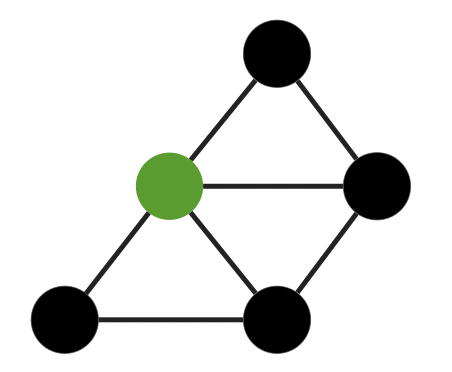
\includegraphics[width=5cm]{schema1.png}
  \caption{A node receives a transaction}
\end{figure}
  
\begin{figure}[htbp]
 \centering
  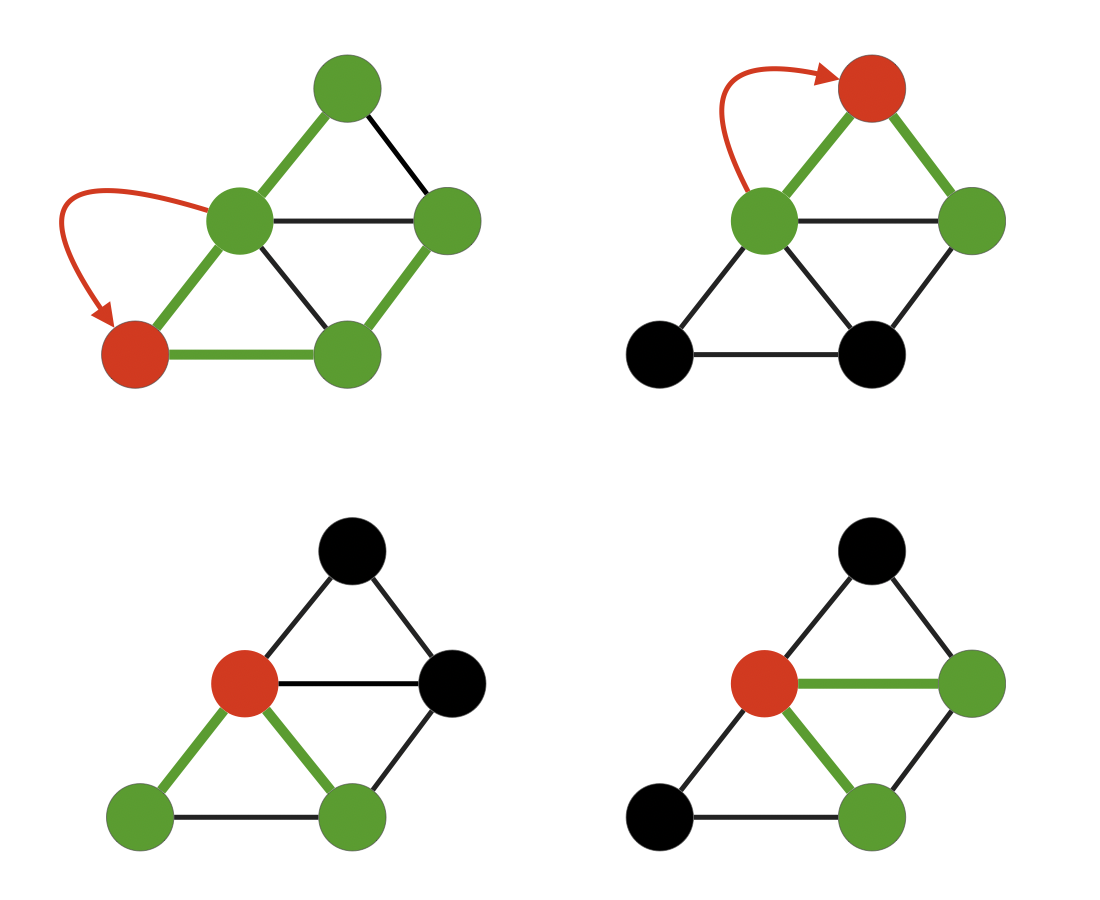
\includegraphics[width=9cm]{schema2.png}
  \caption{The node contacts roots of trees it is a part of. It is also the root of some tree(s)}
\end{figure}

\begin{figure}[htbp]
 \centering
  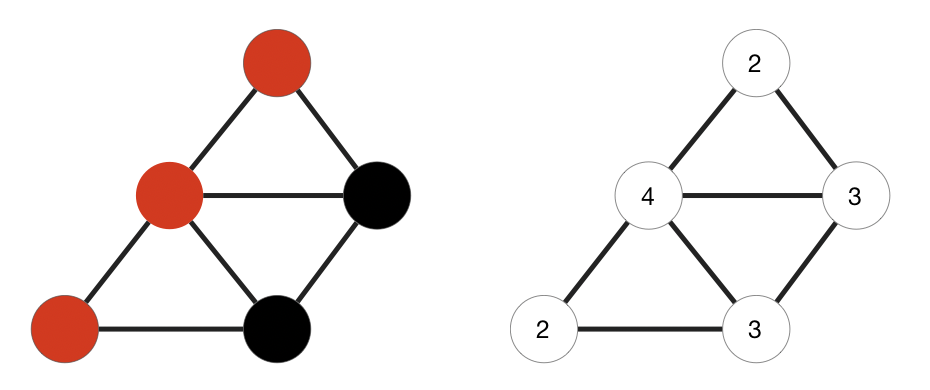
\includegraphics[width=9cm]{schema3.png}
  \caption{Left: roots reached by the process.
   Right: number of signatures received by each node}
\end{figure}


Now that the transactions and signatures have been detailed, the complete process can be explained and exemplified with simple schematics. The overlapping inclusive regions brought up in section 1.1 are translated here to trees and subtrees. Since this section focuses on the general and theoretical design of the project, the details of this translation to trees are not discussed here. More information can be found in section 3.

\newpage

The first node to receive the transaction sends it to the roots of the trees it is a part of, as can be seen in Figure 3.

The root nodes reached seen in Figure 4 all start a consensus for this transaction on their respective trees in parallel. Then, when an aggregate signature is created, the transaction and the signature are propagated on the corresponding tree to be stored individually by each node. This is why every node receives the transaction, but not necessarily every signature. There is always a tree which covers the entire network by definition.

In the very simple example from the figures, the total number of aggregate signatures is 4, since it is the total number of trees the initial node is a part of.

With this system, a node can store different aggregate signatures related to the different regions it is a part of. It will usually receive aggregate signatures of smaller regions first, followed by those corresponding to larger ones.

\subsection{Storage}

We need a storage system which is efficient but keeps every important information. Since a node can receive the same transaction multiple times, it is important to only store each one once. The different signatures should all be stored, since they convey different informations. 

If we only store this however, we cannot easily find the latest transaction for a certain coin and tree, which will often be necessary when testing the correctness of future transactions. To this end, we also keep track of the last transaction for each coin and tree with a lightweight reference. This way, information related to regions is not lost.

It is important to remind that with our transaction design, there is a blockchain for every region and that different coins do not interact with each other. This is why we are storing information ``per coin per tree''.

Before storing a transaction and/or an aggregate signature, the node will first check that the 3 conditions detailed in section 2.1.2 are fulfilled, as well as verify the aggregate signature using the public keys of the corresponding nodes. If the aggregate signature is accepted and stored, the node will mark the corresponding transaction as the latest valid one for this coin and tree.





\section{Implementation}
\label{Implementation}

This section covers how the previously discussed theoretical design was implemented using Cothority, as well as some of the dilemmas faced when building the system. It first touches on the different layers one by one. They are ordered from bottom to top, which happens to be the same order in which they were implemented. The layers are :
\begin{itemize}
\itemsep0em
\item The protocol layer, which validates transactions and generates the aggregate signature
\item The service layer, which launches protocols, store transactions and their signatures as well as propagate them to other services
\item The API layer, which initiates the setup phase of services and sends them transactions
\end{itemize}

\subsection{Protocol}

The only protocol used in this project is the consensus, which collectively signs a transaction. This is the only layer which was already implemented at the start of the project. My work on the protocol was limited to small additions and never changed the fundamental function of the consensus.

The protocol is started on a tree by its root node. When it is finished, the root node updates its public fields indicating if the signing of the transaction was a success as well as the resulting aggregate signature if so. A higher layer can then access those fields.

To check if the 3 transaction conditions detailed in section 2.1.2 are fulfilled, protocol nodes inherits a verification function from the higher layer's service. This function is run in the consensus's prepare phase. If the transaction fails to fulfil the conditions, the node will vote to refuse said transaction.

Those functionalities are resistant against sequential double spending attempts : when a transaction is accepted, the latest valid transaction for this coin is updated and will prevent future transactions coming from the same sender to be accepted by the verification function. With our transaction design, a double spending would be having a particular coin be sent to more than one person.

To prevent concurrent double spending however, something else is needed. Since only one transaction concerning a coin should be handled by a consensus at any given time, we keep track of the availability of every coin atomically. If a node receives a transaction on a coin while it is not done yet with another transaction concerning the same coin for this same tree, it will vote to refuse the last received transaction. Since our system is locality persistent and that a node can simultaneously be part of multiple protocols for different trees, we actually keep track of the availability of every coin for every tree.

\subsection{Service}

The service layer is by far the most important and the one which required the most work for this project. 
Services can start multiple protocols and store the transactions and signatures. Each service pass the verification function (which accesses this service's memory) and the availability of coins per tree to each protocol instance of the same node.

\subsubsection{Service storage}

We use Bbolt \cite{bbolt} for our storing system, which can store byte sequences mapped to keys in multiple buckets. As explained in section 2.4, each node stores the transactions and signatures individually, as well as lightweight references to the latest valid transactions for each coin and tree. The way we do this with Bbolt is having a primary bucket which separately stores each transaction along with its respective signatures. Each key is the hashed encoded transaction. Every encoded structure in this project was obtained with Protobuf \cite{protobuf}, while every hash was computed with the sha256 library. Since the values are byte sequences as well, we also use Protobuf to encode each structure containing the transaction and its signatures before storing them in the first bucket. Protobuf is of course used as well for decoding the byte sequences back into the original structures.

We use a second bucket specifically to store the lightweight references to the latest valid transaction for each coin and tree. The keys are a concatenation of the tree's and coin's identities, while the value is simply the hashed encoded transaction considered as the latest one. Since this is its key in the main bucket, it is easy to access the latest transaction and its aggregate signatures at any given time.

\subsubsection{Setup}

Before normal transactions can be handled by a service, multiple things need to be set up in services.

The nodes, their coordinates and the trees that make up the network are generated with a package that was provided specifically for this project. Services use that package to access a file containing information on the different nodes that make up the network as well as their coordinates. Each service can then deterministically construct the different trees and store which trees it is a part of, as well as the roots of those trees. This will be used to concurrently launch the protocols as described in section 2.3.

Genesis transactions also need to be taken care of for each coin. Each service can directly store genesis information in its buckets which will be needed for the first real transaction to pass the verification function. The receiver of this genesis transaction is the first real ``holder'' of a coin, and can make the first real transaction by sending it to another person.

\subsubsection{Transaction processing}

The implementation closely follows the one described in section 2.3. The first node which learns about a transaction forwards it to the other roots of the trees it is a part of and they all launch the protocol on their trees concurrently. In this project, the first node is contacted via the API (detailed in section 3.3). As soon as a protocol is complete, the service checks if the protocol was successful. If so, it propagates the transaction and the newly created aggregate signature along the tree so that they can be stored. 

The availability of a certain coin per tree, which is shared with the protocols, is only reset after the node receives the propagated transaction and signature. It can also be reset if the protocol fails to accept the transaction. A service will refuse to launch a protocol if the transaction does not pass the verification function or if the coin is not available for that tree.


\subsection{API}
The API layer is relatively straightforward, its most important functionality is sending transactions to individual services. Since services relay received transactions so that they reach the entire network, the client should only contact one service. Services will then automatically handle the usual process of launching parallel consensuses, propagating the results as well as storing them.

The API initiates the setting up phase (section 3.2.2) of services as well. It also sends them the relevant information so that services can store the genesis transactions, namely the coin identity and the public key of the first holder of the coin. It is important to remind that actors are only identified by their public key.

This layer is the only one we take control of when doing simulations. It can also request data from services which is useful in simulations.

\subsection{Tree-based vs set-based storing}

The most interesting dilemma faced when implementing the system was choosing how to store information. Up to this point the translation from the Nyle regions to trees was only brought up briefly. Since we are keeping track of the latest transactions per tree, this means that different trees which spawn the same set of nodes could disagree on the latest transaction. It is not as big an issue as one could think since it is unlikely to happen for big trees and that disagreements should be possible to handle in Nyle. 

However, having a ``set-based'' storing system can have very interesting benefits. We do not store redundant information (trees of same members should agree anyway), which alleviates the memory usage of the secondary bucket and, more importantly, we run less protocols. Keeping track of the latest transaction per set of nodes instead of tree also means that the entire set is marked as available or unavailable with the atomic state of coins. Thus, even without reimplementing much, the general workload of the system is automatically alleviated. Where multiple protocols covering the same set of nodes were happening concurrently (all concerning the same transaction), only one protocol is executed after the change, and its resulting aggregate signature concerns the set as a whole.

This change was actually made in the middle of the project. A system that ``translated'' trees to a byte sequence corresponding to the set was created and used instead of the tree's identity (notably in the secondary bucket keys). The change was made quickly with this translation system but did not involve any real ``in depth'' redesign, which meant that some parts still worked like before and could have been improved or cleaned. Improvements in speed were noticeable nonetheless.

However, some specific cases were more difficult to handle with the set-based system. To limit risks as the project approached its end date, the system was reverted back to tree-based storing. The set-based solution is still available in another branch, and also includes the following functionality:

Every time a node stored a new aggregate signature and marked the transaction to be the latest one for that coin and set, it also marked it as such for every subset of that set. This was intuitive since bigger sets are safer and could alleviate the workload even more in certain cases. However, it resulted in more memory usage in the second bucket which was not always used, and was implemented before nodes contacted the roots of trees they were a part of. This would have required more work since they should ideally not contact roots which spawn trees of similar nodes. The method used to compute subsets was also easier to implement than a method to compute subtrees, which Cothority lacks at the moment.

This functionality is important because it makes successive transactions on a same coin possible in different regions no matter what. Since nodes use the verification function for the specific set on which the protocol is run, it's possible that the verification would refuse a valid transaction because the latest valid transaction wasn't updated for that particular subset.





\section{Simulation analysis}
The chosen analysis focuses on the memory usage of the system. As was explained in section 2.3, every node of the network receives every transaction but not necessarily every aggregate signature. This means that the variations in memory storage between different nodes should only depend on the number of signatures a node receive. 

Since signatures are only propagated to their respective tree, the most important factor determining the memory usage of a node should be the number of trees the node is a part of. The results obtained in simulations should confirm this correlation.

To this end, an API functionality was created. It asks every service for its total Bbolt memory usage as well as the number of trees it is a part of. The client then sorts the different memory usages per ``number of trees a node is a part of'' and computes the average memory for each tree participations number. We expect to see an increase in memory usage for nodes with a higher tree count.

This particular simulation sends 100 transactions which are unrelated because they concern 100 different coins. The transactions are sent from the client to different services, which means that different nodes will relay the transactions. The simulation was done on 3 different networks comprised of 50, 75 and 100 nodes. Nodes are not contacted randomly. For example, each node of the 50 nodes network will receive 2 transaction, while nodes of the 100 nodes network will receive one transaction each from the client.

It is important to detail the size of transactions and signatures in bytes before presenting the results. Each transaction contains :
\begin{itemize}
\itemsep0em
\item The marshalled public key of the sender : 128B
\item The marshalled public key of the receiver : 128B
\item The sender's signature : 64B
\item The coin identity : 1B
\item The reference to the genesis transaction : 1B
\item A payload of dummy data : 650B
\end{itemize}

Each aggregate signature's size is 64B. The Protobuf encoded transactions without payload have a measured size of 350B, which is slightly higher than the sum of their 4 components. This is likely due to the fact that Protobuf also needs data to store information on the transaction's structure itself. The payload was intentionally chosen to bring the total encoded transaction size to 1KB, which simplifies calculations and gives them a more realistic scale compared to the 64B size of aggregate signatures.

The memory results are the difference in storage before and after the transactions are sent, meaning the storage used to store genesis transactions is not taken into account.


\begin{figure}[htbp]
 \centering
  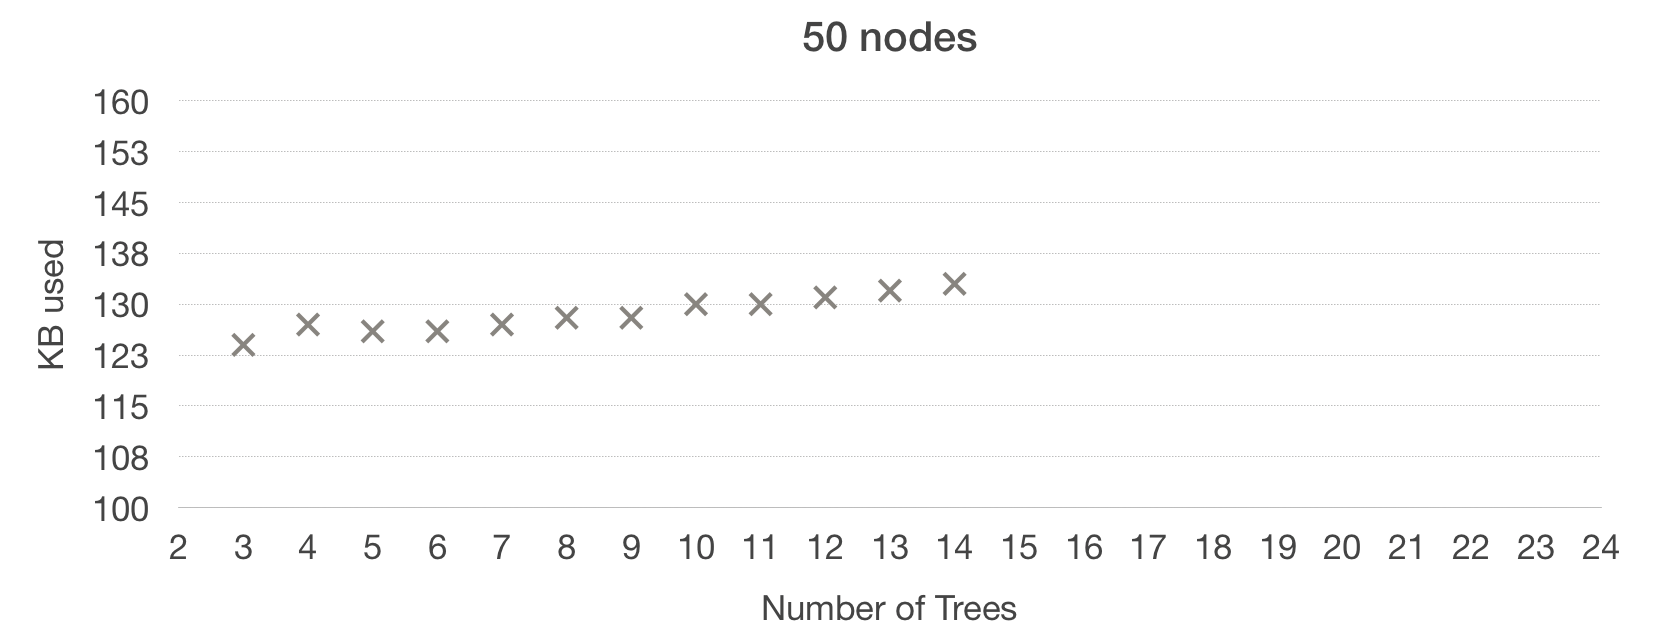
\includegraphics[width=\textwidth]{50graph.png}
  \caption{Average memory usage in a network of 50 nodes}
\end{figure}

\begin{figure}[htbp]
 \centering
  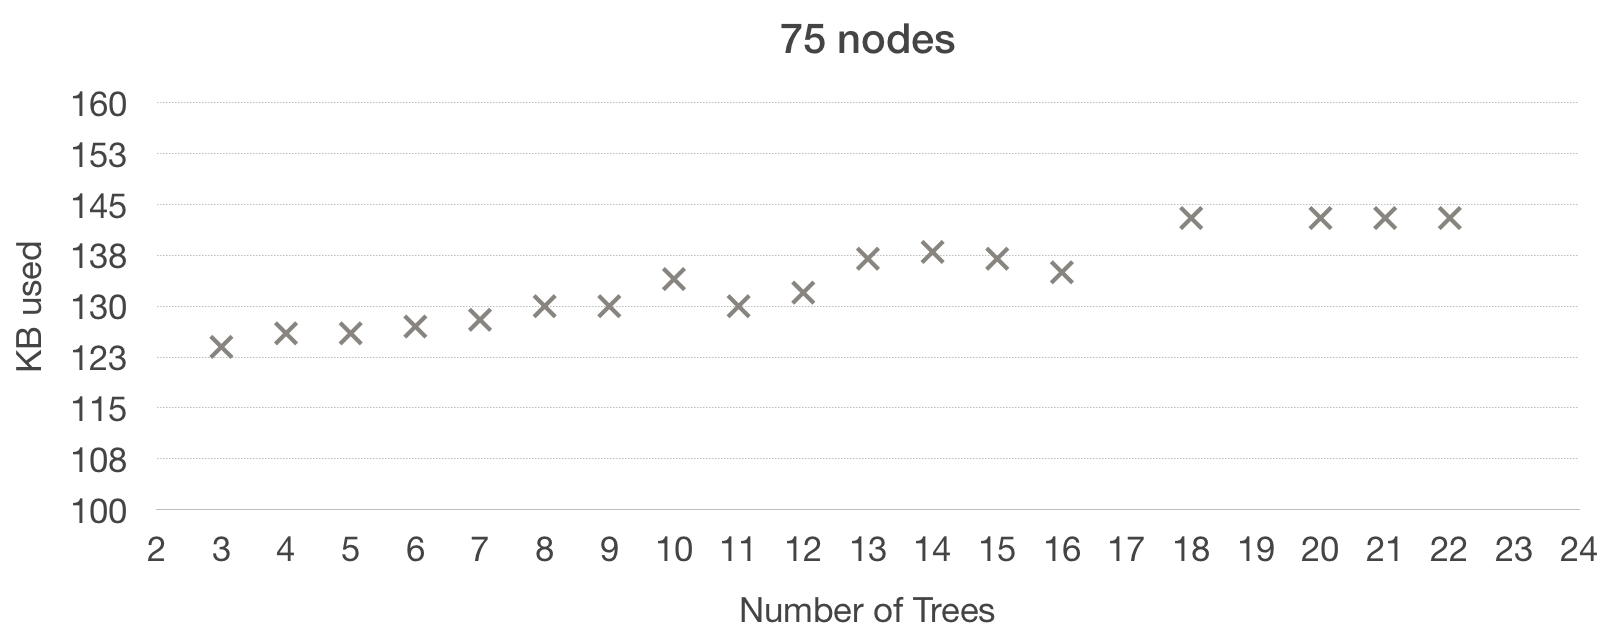
\includegraphics[width=\textwidth]{75graph.png}
  \caption{Average memory usage in a network of 75 nodes}
\end{figure}

\newpage
The storage values start at 100KB, which theoretically corresponds to the memory used by the 100 transactions that every node received. Thus, the charts should only be showing memory used by the aggregate signatures. The fact that the minimum tree count is 3 for the networks of 50 and 75 nodes is a very crucial information. It means that there are 3 trees which spawn the entire set. Thus, the roots of those trees are always contacted in the process and the 3 resulting aggregate signatures will be stored by every node.

The theoretical total storage size that these 3 signatures should take is $100 \times 3 \times 64=19'200$ bytes. This is slightly lower than the 24KB measured for nodes which are part of 3 trees, but is likely due to the fact that Bbolt takes a bit more memory than the theoretical values. We are notably only keeping track of the size of transactions and signatures, while Bbolt also requires memory for the indexes. The 100 indexes of the transactions are hashes of 32B which amount to 3.2KB, which already brings the total number closer to the measured 24KB. We are also not taking metadata into account.

One could naturally wonder why the memory values are not strictly increasing with a higher tree number. The explanation is that while the number of trees a node is a part of is the largest factor in determining memory usage, it is not the only one. Ideally, the size of said trees should be taken into account too because they influence how often they will be reached by the process. This is why nodes with a higher tree count can have a lower average memory usage than nodes with a lower tree count.

The tree sizes are also the reason why the upper bound is only reached for nodes which are only part of the ``full'' trees. For example, the upper bound for a node part of 22 trees in the 75-nodes network should be around $100'000 + 100 \times 22 \times 64 = 240'800$ bytes, which is way higher than the measured
143KB. This is because the 22 trees of which the node is a part of are not always reached, meaning the node receives a lot less than 22 signatures per transaction on average.

We do see an overall increase in memory which clearly confirms the correlation. The reason why the increase is slightly higher for the network of 75 nodes is likely due to how trees are constructed in the  provided package. Increasing the number of nodes without adapting other parameters probably results in bigger trees that are reached more often, thus increasing the storage more on average.

\begin{figure}[htbp]
 \centering
  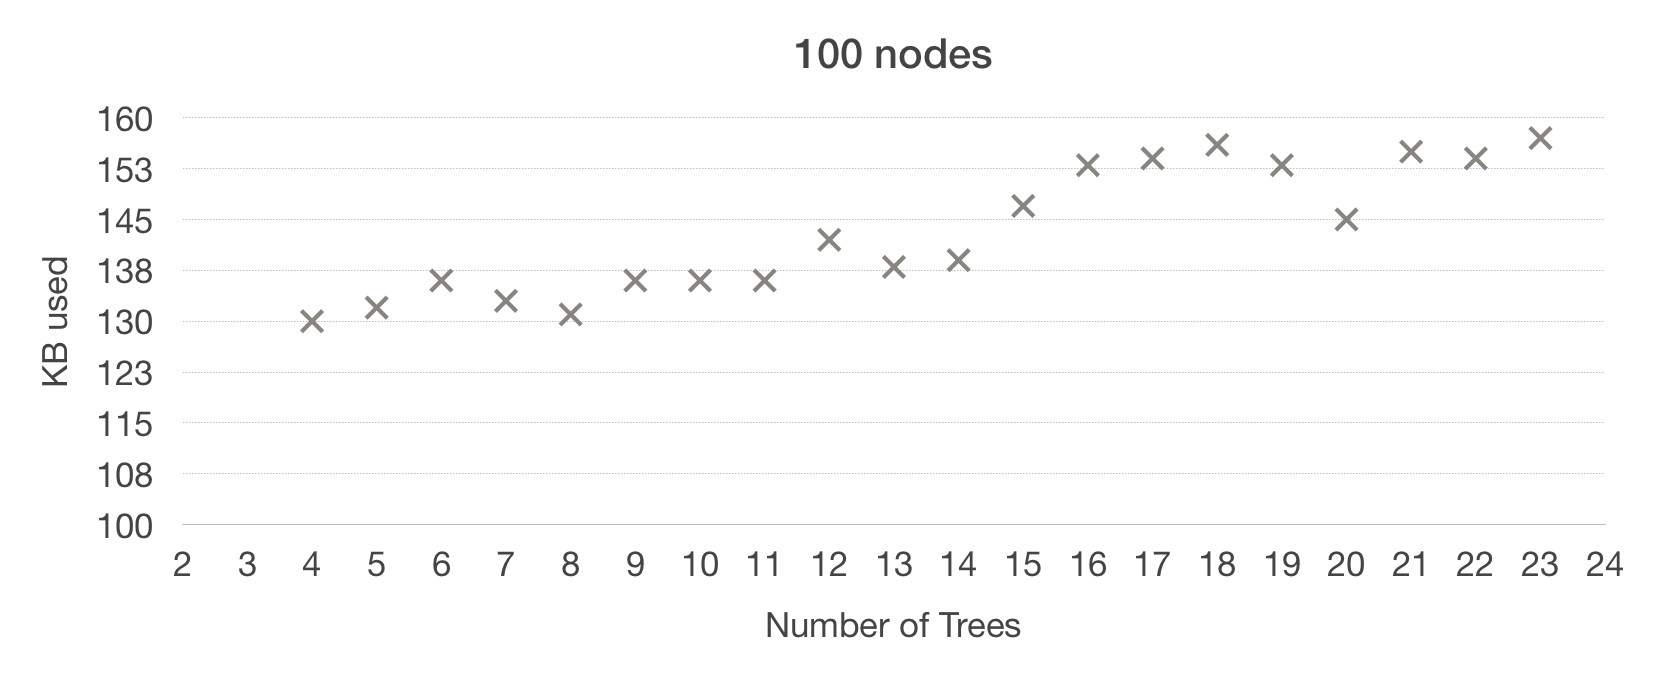
\includegraphics[width=\textwidth]{100graph.png}
  \caption{Average memory usage in a network of 100 nodes}
\end{figure}

\begin{figure}[htbp]
 \centering
  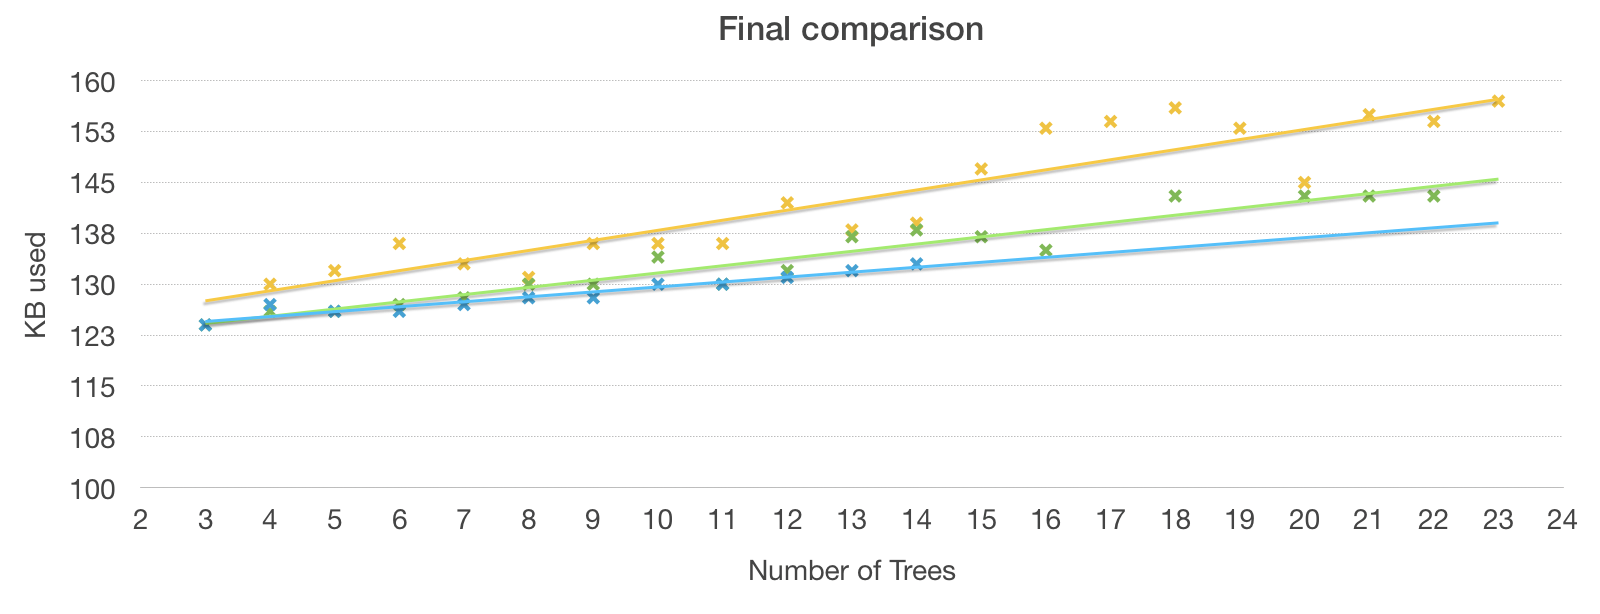
\includegraphics[width=\textwidth]{all3graph.png}
  \caption{Comparison of the 3 previous figures}
\end{figure}


The network of 100 nodes has one important difference compared to the other two : there are 4 trees which spawn the entire set instead of 3. This means that every node will receive one more aggregate signature for each transaction, which should amount to a total memory increase of $100 \times 64 = 6'400$ bytes. Since the memory for nodes part of 4 trees is about 130KB for this network compared to 124KB for nodes part of 3 trees in the previous network, this does seem verified.

The final comparison is satisfying overall, and corresponds to what we would expect. As was brought up previously, the increase in memory is likely higher for larger networks as a result of how trees are constructed in the provided package. The values corresponding to the 100-nodes network (in yellow) are overall higher because every node receives at least 4 signatures, against 3 minimum for the other two networks. 

Even if it is highly dependant on the transaction size to signature size ratio, the system seems to scale well from a storage perspective. The runtimes for executing the 100 transactions sequentially were 2:16, 4:03 and 7:50 for the respective networks of 50, 75 and 100 nodes. This seems to indicate a complexity of $O(n^2)$ at worst, which is not particularly impressive but is to be expected.

The system is also capable of simulating delays based on the distances separating nodes which communicate together. A matrix of distances is created from the nodes's coordinates and is used both by services and protocols. However, this functionality was disabled since the runtimes of these particular simulations are already quite high.

Experimenting with different payload sizes gave expected results. For example, a higher payload of 3650B instead of 650B simply returned the same values  $+300$KB. A chart was not included because of its redundancy.

\section{Future work}
\begin{itemize}
\itemsep0em

\item The next logical step would be to implement the functionality that was done in the set-based storing system (described in section 3.4) in the master branch which uses tree-based storing, as well as analyse what impact this would have on storage by running new simulations. 

\item The actual Go code could be cleaned more. Since new functionalities were implemented up to the very last week, there was not a final ``clean-up phase''. While comments are numerous, the code itself could be touched up for more readability and consistency.

\item Having multiple clients send unrelated transactions concerning different coins to services concurrently does not improve the runtime compared to having one client send transactions sequentially. It would be good to investigate to find the cause. This could allow high scale simulations to be executed more quickly.

\item If the set-based solution is deemed worth prioritising, redesigns should be considered since the system was first implemented with tree-based storing in mind. Each set should probably select a particular tree as its ``representative'' and avoid launching protocols on the others.

\item Run simulations which make use of the distance-based delays, which would be more focused on the runtimes as opposed to the storage.

\end{itemize}


\newpage
\section{Bibliography}
\bibliographystyle{unsrt}
\bibliography{biblio}
\end{document}
